\begin{tcolorbox}[colback=blue!5!white,colframe=blue!75!black,title=PLC]
	Es una computadora que se utiliza en la ingeniería de automatización para controlar procesos las industrias.
\end{tcolorbox}

\subsubsection{Módulos PLC M340}
El laboratorio cuenta con un PLC modular de la marca \textbf{Schneider Electric} de la familia \textbf{Modicon} modelo \textbf{M340} que posee los siguientes módulos:
\begin{itemize}
	\item BMX XBP 0400: bastidor para 4 módulos más la fuente de alimentación.
	\item BMX P34 2030: CPU 340-20 Ethernet CANopen.   (Comunicación)
	\item BMX ART 0414: 4 entradas TC/RTD con separación de potencial.
	\item BMX DDM 16022: 8 entradas digitales, y 8 salidas digitales por transistor PNP, todas ellas aisladas.
	\item BMX CPS 2000: Fuente de alimentación de 220V
\end{itemize}
\begin{center}
	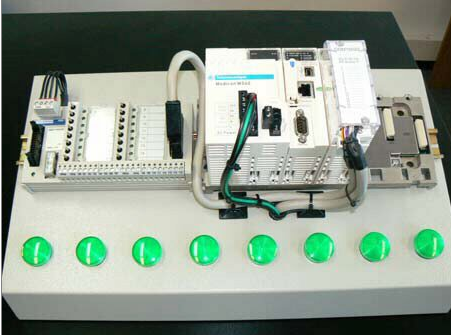
\includegraphics[scale=0.8]{educativo.png}
	\captionof{figure}{Módulo Didáctico PLC M340}
\label{fig:didac}
\end{center}



\subsubsection{Comunicación}
\hl{poner el diagrama}//
\hl{falta leer esto y acomodar}
El   variador   también   se   puede   controlar   en   modo   remoto.   Es   adecuado   paraaplicaciones en   los   que   los   cambios   de   variables   del   variadorse   realizan frecuentemente  durante  el proceso.  Dichos  cambios  pueden  realizarse  por  parte  del propio  operario  (mediante  potenciómetros,  interruptores,  selectores  rotativos  o  BCD, etc.).  Sin  embargo,  la  situación  más  común  es  que  los  parámetros  del  variador  los establezca  el  equipo  de  control  y  supervisión  del  proceso,  al  que  está  conectado  el variadorde  frecuencia: reguladores  de  tensión  y/o  corriente,  finales  de  carrera, pantallas de operador, etc., o incluso un ordenador personal y/o PLC. Para  el  casode  estos  controles  remotos,  la  comunicación  se  puede  realizarde  dos modos:\\Mediante un  número  determinado  de  conductores,  que  depende  de  los elementos que se tengan conectados al variador de frecuencia, por el que se transmiten señales digitales (finalesde carrera, interruptores, salidas digitales de un PLC), o analógicas (potenciómetro, salida analógica de un PLC):\\Mediante un bus de comunicaciones industriales (de 2 o 4 hilos), sobre el que se transmiten   mensajes   de   ajuste   de   parámetros   siguiendo   un   protocolo preestablecido (Modbus, CanBus, ProfiBus, EtherCat, etc.).Con 2  conductores la  comunicación  se  hace  más  lenta(modo  semidúplex),  pero  lógicamente representa un menor coste.

\begin{figure}[htb]
	\centering
	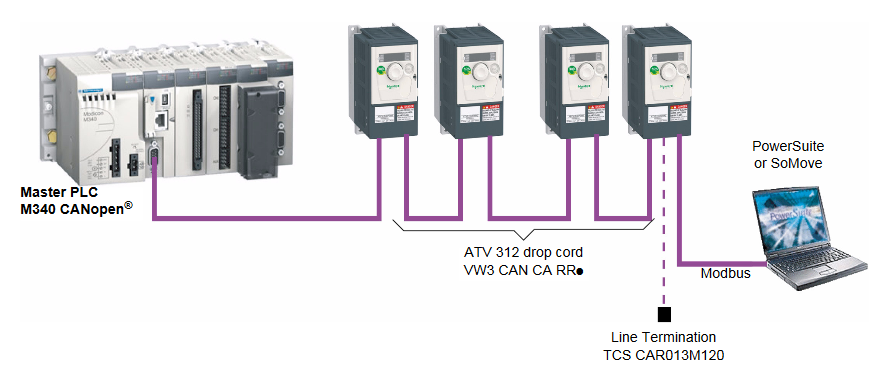
\includegraphics[scale=0.7]{comu.png}
	%\caption{Placa BME280}
	%\label{fig:BME280}
\end{figure}


\paragraph{Configuración CANopen}

\hl{imagenes. y paso a paso}\\
\\

\paragraph{Configuración Modbus}
\begin{tcolorbox}[colback=blue!5!white,colframe=blue!75!black,title=ModBus]
	Modbus es un protocolo de comunicaciones utilizado para transmitir información a través de redes en serie entre dispositivos electrónicos, basado en la arquitectura maestro/esclavo o cliente/servidor, diseñado en 1979 por Modicon para su gama de PLC. Convertido en un protocolo de comunicaciones estándar en la industria. Además, esta red de comunicación industrial usa los protocolos RS232/RS485/RS422.
	%http://microelecblog.blogspot.com/2013/12/configuracion-atv312-para-red-modbus.html
\end{tcolorbox}
\hl{imagenes. y paso a paso}

\subsubsection{Programación Unity Pro}
\begin{tcolorbox}[colback=blue!5!white,colframe=blue!75!black,title=Definición]
	Es una herramienta de configuración, programación y depuración de PLC de la empresa \textbf{Schneider Electric}.
\end{tcolorbox}

\paragraph{Guia}
Para generar la base del proyecto para trabajar, se debe descargar desde la página oficial e instalar el software Unity Pro XL y la librería DTM utilizada anteriormente en el software soMove. Una vez que esto está instalado se abre un nuevo proyecto y se configura como se muestra a continuación.
\begin{enumerate}
	\item Se selecciona el bastidor que se posee y los módulos (Figura \ref{fig:uni1}, (Figura \ref{fig:uni0}).
	
	\item 
  \end{enumerate}
\hl{poner las figuras aparte}
	\begin{center}
		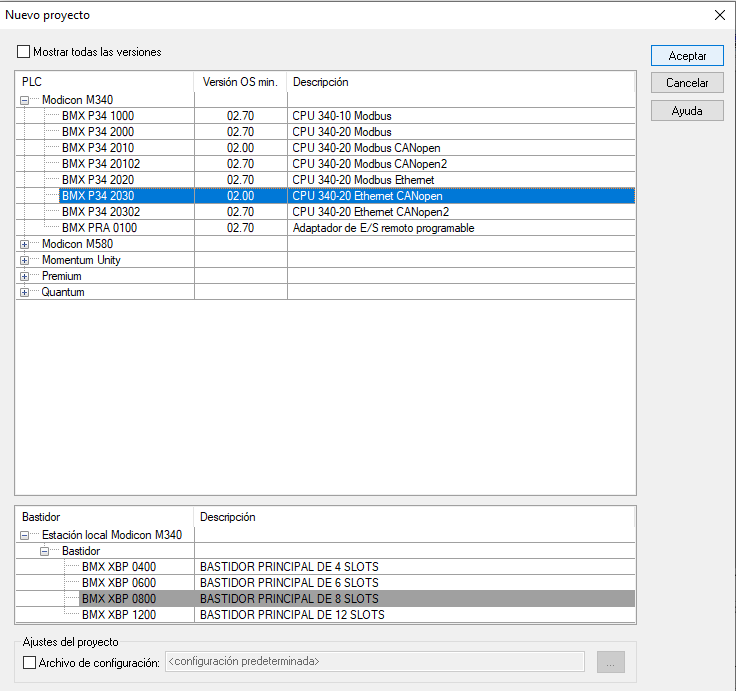
\includegraphics[scale=0.25]{unit1.png}
		\captionof{figure}{Elección del bastidor}
	\label{fig:uni1}
		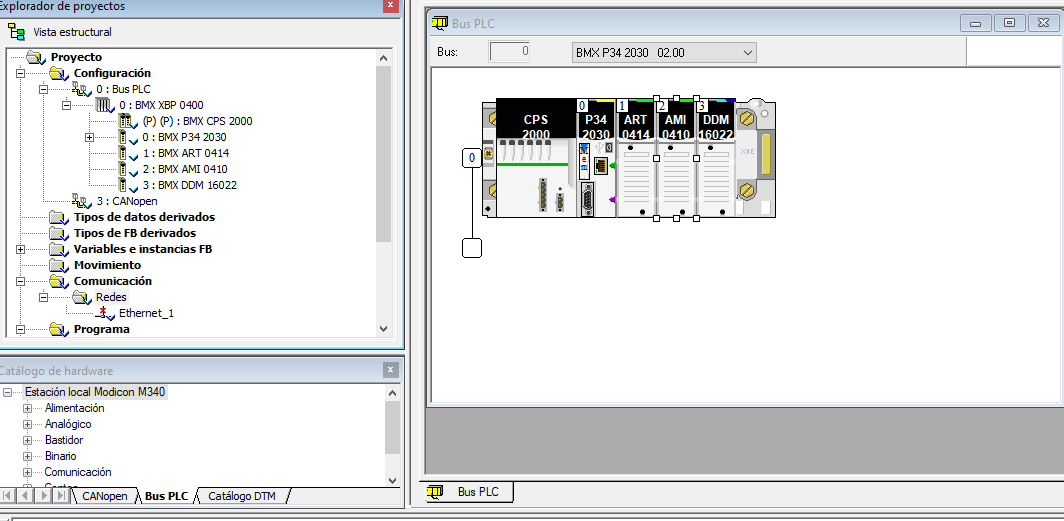
\includegraphics[scale=0.25]{unity1.png}
	\captionof{figure}{Módulos PLC}
	\label{fig:uni0}
	\end{center}
	
	


\paragraph{Programa básico}
\newpage

%EL ERROR QUE TENIA CRISTIAN con ifix SE ARREGLO CON ESTO
%\url{http://www.cimexcorp.com/hasp_fix.htm}